\documentclass[hidelinks,  a4paper, 14pt]{report}
\usepackage[utf8]{inputenc}
\usepackage{graphicx}
\usepackage{hyperref}
\usepackage{vcell}
\usepackage{colortbl}


\title{Analisi \textit{Calzolaio}}
\author{Simone Pozzebon}
\begin{document}
\maketitle
\tableofcontents
\newpage

\section{TESTO DEL PROBLEMA}
\begin{center}
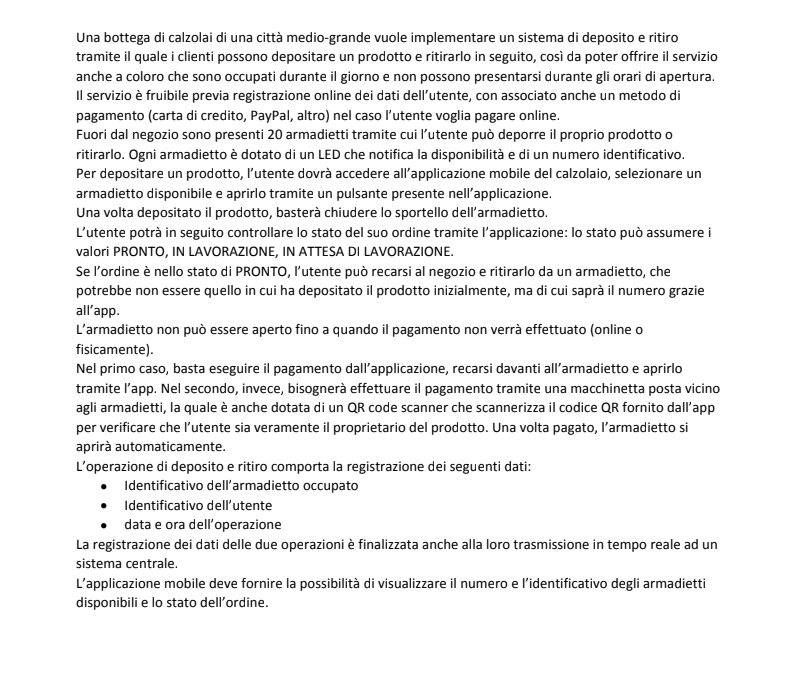
\includegraphics[scale=0.4]{img/2021-03-23-081439_796x698_scrot.png}
\end{center}

\section{ANALISI DELLE ENTITA'}
\subsection{Entita'}
Le Entità che possono essere individuate nel problema sono: 
\begin{itemize}
\item \textit{Persona}, identifica i dati anagrifici degli utenti del sito;
\item \textit{Account}, identica i veri e propri account del sito;
\item \textit{Pagamento}, riferisce a tutte le caratteristiche di un pagamento approvato o in attesa di approvazione;
\item \textit{Ordine}, identifica tutte le caratteristiche di un ordine effettuato.
\end{itemize}
\newpage
\subsection{Diagramma E/R}
\begin{center}
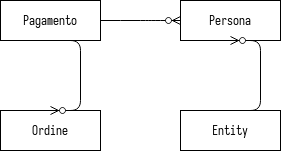
\includegraphics[scale=0.5]{img/erCalzolaio.png}
\end{center}

\subsection{Schema Logico}
    \subsubsection{Tabelle}

        \begin{enumerate}
            \item pagamento(\underline{idPagamento}, transazione, ammontare, causale);
            \item ordine(\underline{idOrdine}, * lavorazione, ordine, tempoAttesa);
            \item account(\underline{idAccount}, * user, password);
            \item persona(\underline{idPersona}, nome, cognome, email , dataRegistrazione, indirizzo);
        \end{enumerate}
\newpage

\end{document}


